\documentclass[A4,12PT, english, twocolumn]{journal}
\usepackage{amsmath,amssymb,amsfonts}
\usepackage[margin=0.7in]{geometry}
\usepackage{graphicx}
\usepackage{enumitem}
\usepackage{xcolor}
\usepackage{hyperref}
\usepackage{tabularray}
\usepackage{multicol}
\usepackage{tikz}
\usepackage{circuitikz}
\usepackage{scalerel}
\usepackage{pict2e}
\usepackage{tkz-euclide}
\usetikzlibrary{calc}
\usetikzlibrary{patterns,arrows.meta}
\usetikzlibrary{shadows}
\usetikzlibrary{external}

%pgfplots
\usepackage{pgfplots}
\pgfplotsset{compat=newest}
\usepgfplotslibrary{statistics}
\usepgfplotslibrary{fillbetween}

\def\infinity{\rotatebox{90}{8}}

% Hiperlink
\hypersetup{
    colorlinks=true,
    linkcolor=blue,
    filecolor=magenta,      
    urlcolor=cyan,
    pdftitle={Overleaf Example},
    pdfpagemode=FullScreen,
}
%\usepackage{style}
\NewDocumentCommand{\Log}{o}{%
\IfNoValueTF{#1}{}{{}^{#1}\!}\log}%
  
%command buat logaritma dengan basisnya di pojok kiri
%\textheight=17cm
%\textwidth=10cm
%\usepackage{blindtext}
\setenumerate[1]{itemsep=0,5cm}
\setenumerate[2]{topsep=5pt, itemsep=5pt, label=\textbf{\Alph*}.}

\title{Matematika Saintek \& Fisika UTUL UGM 2019 Kode 924}
\author{Fauzan Akbar Sukandar Putra \\ \LaTeX}

\begin{document}

\maketitle

%\begin{minipage}{0.5\textwidth}
\begin{enumerate}
%1%
\item Sebuah kotak memuat $6$ bola merah dan $4$ bola hitam. Tiga bola diambil satu per satu tanpa pengembalian. Jika bola ketiga terambil merah, maka banyak kemungkinannya adalah\dots
    \begin{enumerate}
        \item $234$ 
        \item $243$
        \item $324$
        \item $342$
        \item $432$
    \end{enumerate}
  
%2%
\item Diketahui penyelesaian dari pertidaksamaan $\frac{3^{x+3}+3^x-36}{9^x-9}\leq3$ adalah $a\leq x< b$ atau
$x \geq c$. Nilai $a+2b+c=$\dots
    \begin{enumerate}
        \item $0$
        \item $1$
        \item $2$
        \item $3$
        \item $4$
    \end{enumerate}
     
%3% 
\item Jika $a<x<b$ adalah solusi dari pertidaksamaan\\$1+2^x+2^{2x}+2^{3x}...>2$, dengan $x \neq 1$, maka $a+b=\dots$
    \begin{enumerate}
        \item $-1$
        \item $-2$
        \item $-3$
        \item $-4$
        \item $-5$
    \end{enumerate}
   
%4%
\item Diberikan lingkaran pada bidang koordinat dengan titik pusat $(a,b)$ dan memotong sumbu-X di titik $(3,0)$ dan $(9,0)$. Jika garis yang melalui titik $(0,3)$ menyinggung lingkaran di titik $(3,0)$, maka nilai dari $a^2-b^2$ adalah\dots
    \begin{enumerate}
        \item $9$
        \item $18$
        \item $27$
        \item $36$
        \item $45$
    \end{enumerate}

%5%
\item Jika $(x-2)^2$ membagi $x^4-ax^3+bx^2+4x-4$,\\maka $ab=\dots$
    \begin{enumerate}
        \item $9$
        \item $12$
        \item $16$
        \item $20$
        \item $25$
    \end{enumerate}
    
%6% 
\item Diberikan empat matriks $A,B,C,D$ berukuran $2\times 2$ dengan $A+CB^T=CD$. Jika $A$ mempunyai invers, $\det (D^T-B)=m$ dan $\det (C)=n$. maka $\det (2A^{-1})=\dots$
    \begin{enumerate}
        \item $\frac{4}{mn}$
        \item $\frac{mn}{4}$
        \item $\frac{4m}{n}$
        \item $4mn$
        \item $\frac{m+n}{4}$
    \end{enumerate}
    
%7%
\item Jika $-\frac{\pi}{2}<x<\frac{\pi}{2}$ dan $x$ memenuhi \\ $5\cos^2x+3\sin x \cos x \geq 1$ maka himpunan semua \\ $y=\tan x$ adalah\dots
    \begin{enumerate}
        \item $\{y \in R:-1 \leq y \leq 4\}$
        \item $\{y \in R:-4 \leq y \leq 1\}$
        \item $\{y \in R:-4 \leq y \leq -1\}$
        \item $\{y \in R:1 \leq y \leq 4\}$
        \item $R$
    \end{enumerate}
    
%8%
\item Jika suku banyak $x^4+3x^3+Ax^2+5x+B$ dibagi \\ $x^2+2x+2$ bersisa $7x+14$, maka jika dibagi $x^2+4x+4$ akan bersisa\dots
    \begin{enumerate}
        \item $x+1$
        \item $x+2$
        \item $x+3$
        \item $2x+1$
        \item $2x+4$
    \end{enumerate}
    
%9%
\item Jika
\begin{center}
    \begin{cases}
        $(^2\Log x)^2-(^2\Log y)^2=\;^2\Log 256$\\
        $^2\Log x^2-^2\Log y^2=\;^2\Log 16$,
    \end{cases}
\end{center}
maka nilai dari $^2\Log x^6y^{-2}$ adalah\dots
	\begin{enumerate}
		\item $24$
		\item $20$
		\item $16$
		\item $8$
		\item $4$
	\end{enumerate}
	
%10%
\item Diberikan kubus $ABCD.EFGH$ dan $P$ adalah titik tengah $BC$. Perbandingan luas segitiga $APG$ dan luas segitiga $DPG$ adalah\dots
   \begin{enumerate}
        \item $1:1$
        \item $\sqrt{3}:\sqrt{2}$
        \item $\sqrt{2}:1$
        \item $3:2$
        \item $\sqrt{3}:1$
   \end{enumerate}
   
%11%
\item Misalkan $U_n$ menyatakan suku ke-$n$ dari barisan aritmatika. Diketahui $U_1 \times U_2 = 10$ dan $U_1 \times U_3 = 16$. Jika suku-suku dari barisan aritmatika tersebut merupakan bilangan positif, maka $U_{10}=\dots$
    \begin{enumerate}
        \item $21$
        \item $23$
        \item $25$
        \item $27$
        \item $29$
    \end{enumerate}
  
%12%
\item Diketahui fungsi $f$ dan $g$ dengan $f(x)=(2x+1)^5$ dan $h = f \circ g$. Jika $g(5) = -1$ dan $g'\left(\frac{x+1}{x-1}\right)=2x+2$, maka $h'(5)=\dots$
    \begin{enumerate}
        \item $10$
        \item $25$
        \item $50$
        \item $60$
        \item $120$
    \end{enumerate}
    
%13%
\item Jika $p>0$ dan $\lim\limits_{x \to p}\frac{x^3+px^2+qx}{x-p}=12$, maka nilai $p-q$ adalah\dots
    \begin{enumerate}
        \item $14$
        \item $10$
        \item $8$
        \item $5$
        \item $3$
    \end{enumerate}

%14%
\item Jika $\sin{x}+\sin{2x}+\sin{3x}=0$ untuk $\frac{\pi}{2}<x<\pi$, maka $\tan{2x}=\dots$
    \begin{enumerate}
        \item $-\sqrt{3}$
        \item $-1$
        \item $-\frac{1}{3}\sqrt{3}$
        \item $\frac{1}{3}\sqrt{3}$
        \item $\sqrt{3}$
    \end{enumerate}

%15%  
\item Diketahui 
\begin{center}
    \begin{cases}
        $x^2+2xy+4x=-3$\\
        $9y^2+4xy+12y=-1$\\
    \end{cases}\\
\end{center}
Nilai dari $x+3y$ adalah\dots
\begin{enumerate}
       \item $2$
       \item $1$
       \item $0$
       \item $-1$
       \item $-2$
    \end{enumerate}
    

%FISIKA %
%16%
\newpage
\item Sebuah benda bergerak sepanjang garis lurus dengan kecepatan sebagai fungsi waktu diperlihatkan pada gambar. Diantara pernyataan-pernyataan berikut ini, mana yang benar?
\begin{center}
    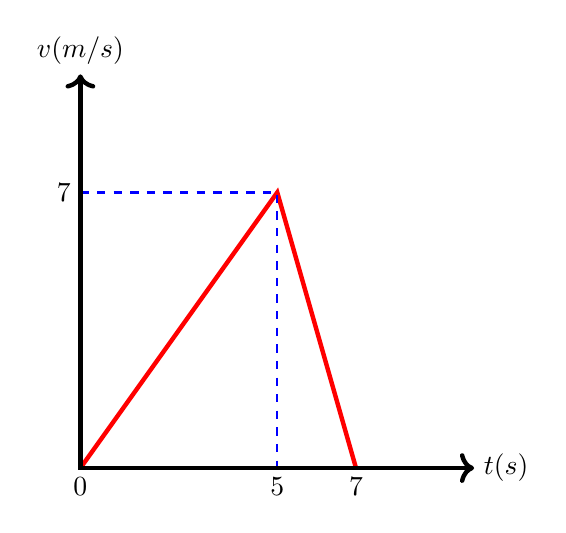
\begin{tikzpicture}[scale=0.5]
        %GRID
        %\draw[lightgray] (0,0) grid (10,10);

        %GRAFIK
        \draw[red, ultra thick] (0,0) -- (5,7) -- (7,0);

        %GARIS BANTU
        \draw[dashed, blue, thick] (0,7) -- (5,7) -- (5,0);

        %AXIX
        \draw[ultra thick, <->] (10,0) -- (0,0) -- (0,10);

        %LABEL
        \node[left] at (0,7){$7$};
        \node[below] at (5,0){$5$};
        \node[below] at (7,0){$7$};
        \node[below] at (0,0){$0$};
        \node[right] at (10,0){$t(s)$};
        \node[above] at (0,10){$v(m/s)$};
    \end{tikzpicture}
\end{center}
    \begin{enumerate}
        \item Tepat setelah $t=5s$, arah gaya berlawana dengan arah gerak benda.
        \item Tepat setelah $t=5s$, kecepatan benda masih searah dengan percepatan benda.
        \item Benda mengalami perlambatan senilai $2,5m/s^2$ saat $t=6s$.
        \item Jarak yang ditempuh oleh benda dari $t=0s$ sampai $t=5s$ adalah $35$ meter.
        \item Percepatan benda mencapai nilai maksimum saat $t=5s$.
    \end{enumerate}
  
%17%
\item Untuk mendapatkan panjang gelombang de Broglie $500 \; nm$, elektron perlu dipercepat dari keadaan diam dengan beda potensial sebesar \dots
    \begin{enumerate}
        \item $2\mu V$
        \item $6\mu V$
        \item $12\mu V$
        \item $38\mu V$
        \item $42\mu V$
    \end{enumerate}
     
%18%
\item Sebuah truk bermassa $1000 \; kg$ melaju dengan kelajuan konstan $100 \; km/jam$ menaiki tanjakan miring dengan kemiringan $\tan{\alpha} = 0,1$. Jika gaya gesekan total yang bekerja pada truk adalah $700 \; N$, hitunglah daya minimum yang harus diberikan oleh mesin truk $\left(g= 9,81 \; m/s^2 \right)$
    \begin{enumerate}
        \item $47,1 \; kW$
        \item $52,7 \; kW$
        \item $62,5 \; kW$
        \item $72,8 \; kW$
        \item $85,1 \; kW$
    \end{enumerate}
   
%19%
\item Dua buah pegas identik, jika terpasang paralel dibutuhkan usaha sebesar $W$ untuk menarik pegas supaya bertambah panjang sebesar $x$. Kemudian keduanya dipasang secara seri. Berapakah usaha yang dibutuhkan pegas yang tersusun seri tersebut agar kedua pegas tertekan sebesar $x$?
    \begin{enumerate}
        \item $\frac{W}{4}$
        \item $\frac{W}{2}$
        \item $W$
        \item $2W$
        \item $4W$
    \end{enumerate}

%20%
\item Tinjau suatu benda yang memiliki massa jenis $\rho_{0}$. Jika benda tersebut dimasukkan ke dalam fluida maka sebanyak $3/4$ bagian volumenya tercelup di dalam fluida tersebut. Hitunglah massa jenis fluida!
    \begin{enumerate}
        \item $\rho_{0}$
        \item $\frac{2\rho_{0}}{3}$
        \item $\frac{3\rho_{0}}{2}$
        \item $\frac{3\rho_{0}}{4}$
        \item $\frac{4\rho_{0}}{3}$
    \end{enumerate}
    
%21%
\item Sebuah gelombang transversal menjalar dengan laju $v$ pada sebuah tali yang memiliki tegangan tali $T$. Berapakah tegangan tali yang dibutuhkan agar gelombang menjalar dengan laju $\frac{2v}{3}$?
    \begin{enumerate}
        \item $\frac{9}{4}T$
        \item $\frac{5}{4}T$
        \item $\frac{11}{9}T$
        \item $\frac{7}{9}T$
        \item $\frac{4}{9}T$
    \end{enumerate}
    
%22%
\item Sebuah silinder berpiston berisi gas ideal yang volumenya $2 \; m^3$, tekanannya $10^5 \; Pa$ dan suhunya $300 \; K$. Silinder itu kemudian disentuhkan pada tandon kalor yang suhunya dijaga tetap pada $900 \; K$. Gas mengalani ekspansi pada tekanan tetap sehingga suhunya menjadi $900 \; K$. Jika perubahan energi internal gas adalah $6 \times 10^5 \; J$, maka berapakah kalor yang diserap oleh gas?
    \begin{enumerate}
        \item $0 \; J$
        \item $4 \times 10^5 \; J$
        \item $6 \times 10^5 \; J$
        \item $8 \times 10^5 \; J$
        \item $10 \times 10^5 \; J$
    \end{enumerate}
    
%23%
\item Sebuah sel surya memiliki efisiensi $\eta$. Luas panelnya adalah $40 \; cm^2$ dan panel tersebut menerima sinar matahari dengan intensitas $10^3 \; W/m^2$. Sel tersebut menghasilkan arus $0,4 \; A$ dengan tegangan $2 \; V$. Berapakah efisiensi $\eta$?
    \begin{enumerate}
        \item $25\%$
        \item $20\%$
        \item $15\%$
        \item $10\%$
        \item $5\%$
    \end{enumerate}
    
%24%
\item Perhatikan wilayah tertutup dalam ruang yang dibatasi oleh suatu permukaan tertutup. Jika garis-garis gaya medan listrik yang menembus masuk pada permukaan itu sama dengan yang menembus keluar, maka \dots
	\begin{enumerate}
		\item Kuat medan listrik pada permukaan itu nol
		\item Kuat medan listrik pada permukaan itu tetap
		\item Potensial listrik pada permukaan itu nol
		\item Potensial listrik pada permukaan tetap
		\item Muatan listrik di dalam permukaan itu nol
	\end{enumerate}
	
%25%
\item Dalam sebuah awan mendung, bagian atas awan bermuatan positif dan bagian bawah negatif karena induksi oleh muatan bumi. Bagian atas awan bisa bermuatan sebesar $+40C$, sedangkan bagian bawah bisa bermuatan $-40C$. Bila muatan-muatan tersebut terpisah sejauh $2 \; km$. Berapakah gaya elektrostatik antara keduanya?
   \begin{enumerate}
        \item $3,6 \times 10^4 \; N$
        \item $3,6 \times 10^5 \; N$
        \item $3,6 \times 10^6 \; N$
        \item $3,6 \times 10^7 \; N$
        \item $3,6 \times 10^8 \; N$
   \end{enumerate}
   
%26%
\item Dua buah bola masing-masing bermassa 1 gram diberi muatan yang sama besar lalu diletakkan sejauh $3 \; cm $ satu dengan yang lain. Ketika dilepaskan masing-masing bola mengalami percepatan sebesar $144 \; m/s^2$. Berapakah besar muatan yang diberikan pada masing-masing bola?
    \begin{enumerate}
        \item $6,4 \times 10^{-7} \; C$
        \item $3,6 \times 10^{-7} \; C$
        \item $2,5 \times 10^{-7} \; C$
        \item $1,2 \times 10^{-7} \; C$
        \item $8,0 \times 10^{-7} \; C$
    \end{enumerate}
  
%27% 
\item Kawat berarus berada di dalam medan magnet sepanjang $50 \; cm$. Arah kawat tegak lurus terhadap medan magnet.Ketika kawat dialiri arus $10 \; A$, resultan gaya pada kawat terukur sebesar $3 \; N$. Berapakah kuat medan magnet yang mempengaruhi kawat berarus ini?
    \begin{enumerate}
        \item $1,8 \times 10^{-3} \; T$
        \item $4,4 \times 10^{-2} \; T$
        \item $0,6 \; T$
        \item $1,4 \; T$
        \item $5,2 \; T$
    \end{enumerate}
    
%28%
\item Seberkas cahaya datang sejajar sumbu utama sebuah lensa cembung sehingga dibiaskan mengumpul di titik apinya. Jika di depan lensa cembung itu diletakkan lensa cekung, maka kemungkinan yang terjadi adalah \dots
    \begin{enumerate}
        \item Berkas dibiaskan dan mengumpul di titik yang lebih jauh
        \item Berkas dibiaskan dan mengumpul di titik yang lebih dekat
        \item Berkas dibiaskan dan mengumpul di titik api lensa cembung
        \item Berkas dibiaskan menyebar seolah berasal dari titik api lensa cembung
        \item Berkas dibiaskan menyebar seolah berasal dari titik api lensa cekung
    \end{enumerate}

%29%
\item Suatu lubang disinari berkas cahaya dengan panjang gelombang $\lambda = 500 \; nm$. Jika jejari lubang sebesar \\ $a = 400\lambda$, maka lebar pola terang tengah yang terlihat pada layar sejauh $1 \; m$ dari lubang adalah sebesar \dots
\begin{enumerate}
        \item $0,5 \; mm$
        \item $1 \; mm$
        \item $2 \; mm$
        \item $5 \; mm$
        \item $10 \; mm$
    \end{enumerate}

%30%
\item Panjang lintasan optik bagi seberkas cahaya adalah perkalian antara panjang lintasan dalam medium dan indeks bias medium itu. Dalam suatu medium yang seragam, lintasan optik paling panjang berarti \dots
    \begin{enumerate}
        \item Juga lintasan yang paling panjang dalam medium
        \item Justru lintasan yang paling pendek dalam medium
        \item Lintasan yang melengkung
        \item Lintasan yang lurus
        \item Lintasan yang patah-patah
    \end{enumerate}

 %31%
\item Untuk melihat sebuah benda yang berada di suatu tempat, lensa mata harus berakomodasi maksimum. Dalam keadaan tanpa berakomodasi, bayangan benda itu \dots
    \begin{enumerate}
        \item Berada di belakang retina dan terbalik
        \item Berada di belakang retina dan tegak
        \item Berada di depan retina dan terbalik
        \item Berada di depan retina dan tegak
        \item Berada di retina dan terbalik
    \end{enumerate}

%32%
\item Seorang pengamat bergerak dengan kecepatan $0,6 \; c$ menyusuri permukaan bumi, dengan $c$ adalah cepat rambat cahaya dalam ruang hampa. Pengamat itu melewati subuah bangun di bumi yang terlihat olehnya sebagai sebuah lingkaran dengan jari-jari $1 \; m$. Bangun geometris itu jika dilihat oleh orang yang diam di bumi berupa elips dengan jarak antar titik api?
    \begin{enumerate}
        \item $0,64 \; m$
        \item $0,75 \; m$
        \item $1,50 \; m$
        \item $1,60 \; m$
        \item $1,82 \; m$
    \end{enumerate}

%33%
\item Hasil eksperimen efek Compton adalah \dots
    \begin{enumerate}
        \item Mendukung pandangan bahwa cahaya adalah partikel
        \item Mendukung pandangan bahwa cahaya adalah gelombang
        \item Memperlihatkan bahwa cahaya tidak memiliki momentum
        \item Intensitas cahaya terkait dengan amplitudo
        \item Frekuensi cahaya berkaitan dengan intensitasnya
    \end{enumerate}

%34%
\item Foton dari cahaya $A$ mempunyai energi dua kali dari energi foton cahaya $B$. Perbandingan energi foton dari cahaya $A$ dengan energi foton dari cahaya $B \; \left(\frac{P_A}{P_B} \right)$ adalah \dots
    \begin{enumerate}
        \item $\frac{1}{4}$
        \item $\frac{1}{2}$
        \item $1$
        \item $2$
        \item $4$
    \end{enumerate}

%35%
\item Menurut teori atom Bohr, jika jejari orbit elektron pada keadaan $n=1$ adalah $0,0529 \; nm$. Berapakah jejari elektron pada keadaan $n=5$ \dots
    \begin{enumerate}
        \item $2,42 \; nm$
        \item $1,32 \; nm$
        \item $0,846 \; nm$
        \item $0,265 \; nm$
        \item $0,106\; nm$
    \end{enumerate}

\end{enumerate}
\end{document}  
